\section{Инструкции за употреба на проекта}
След стартиране на програмата, потребителят трябва да въведе име и парола за вход. Ако това е първото влизане в системата, потребителят трябва да въведе името "admin" и паролата "admin" за вход в администраторския профил. (Фиг. \ref{fig:login}) Тези данни за автентикация могат да бъдат сменени по-късно.

\begin{figure}[H]
    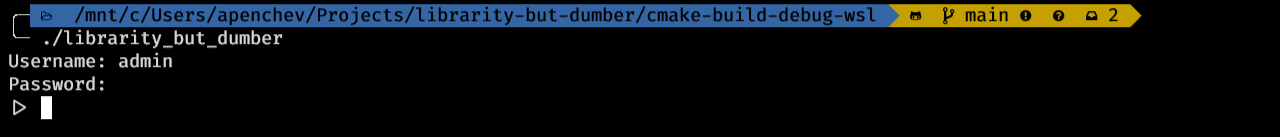
\includegraphics[width=1\textwidth]{1-login.png}
    \centering
    \caption{Вход в системата}
    \label{fig:login}
\end{figure}

След вход в системата, на потребителя се предоставя команден интерфейс, чрез който потребителя може да управлява информацията за книгите и потребителите. При получаване на командата "help", на потребителят се предоставя списък с всички команди, които могат да бъдат използвани. При получаване на командата "exit" или стандартна комбинация Ctrl+D за "приключване на входа", програмата се затваря. Основните команди поддържани от системата са:
\begin{enumerate}
    \item Команда за добавяне на потребител - "add user"
    
    Изисква потедбителят да има администраторски права. При извикване, изисква от потребителя да подаде на стандартния вход име и парола на потребителя, който ще бъде добавен в системата. Също така пита относно това, дали профила да има администраторски права или - не. (Фиг. \ref{fig:add-user})
    \begin{figure}[H]
        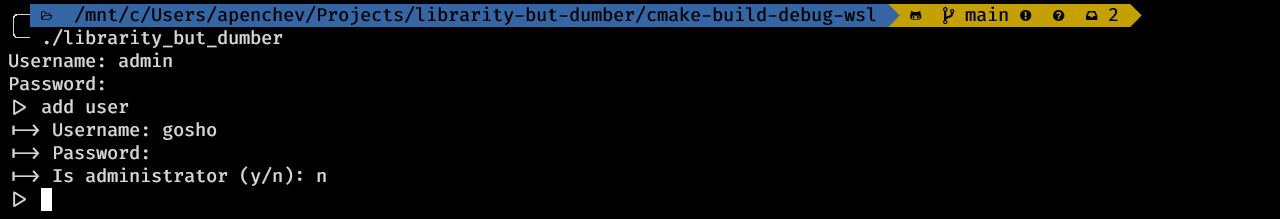
\includegraphics[width=1\textwidth]{2.add-user.png}
        \centering
        \caption{Добавяне на потребител в системата}
        \label{fig:add-user}
    \end{figure}
    
    \item Команда за смяна на паролата - "change password"
    
    При извикване, изисква от потребителя старата му парола, нова парола и повторена нова парола. При несъответствие на паролите, потребителят се показва съобщение за грешка. При валидно промяна на паролата, потребителят се показва съобщение за успешно промяна на паролата. (Фиг. \ref{fig:change-password})
    \begin{figure}[H]
        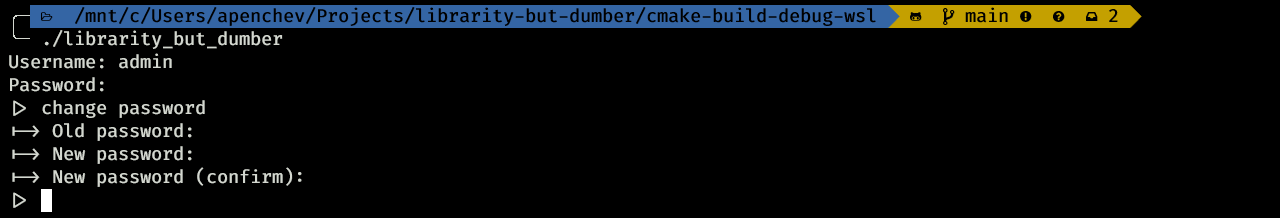
\includegraphics[width=1\textwidth]{3.change-password.png}
        \centering
        \caption{Смяна на потребителската парола}
        \label{fig:change-password}
    \end{figure}
    
    \item Команда за добавяне на книга - "add book" или "add"
    
    Изисква потедбителят да има администраторски права. При извикване, потребителят трябва да подаде на стандартния вход всичката информация нужна за създаванете на книга - име, автор, описание, рейтинг, международен стандартен номер (ISBN) и файлов път, където ще се запази текста на книгата. Ако на файловия път вече съществува файл, потребителя се запитва дали да презапише съдържанието му. След това, на потребителя се дава възможност да избере начин за създаване на файла със съдържанието на книгата - да създаде празен файл, да създаде файл и да го попълни от стандартния вход (Фиг. \ref{fig:add-book-from-cin}) или да създаде файл и да го попълни със съдържанието на друг файл. (Фиг. \ref{fig:add-book-from-file})
    \begin{figure}[H]
        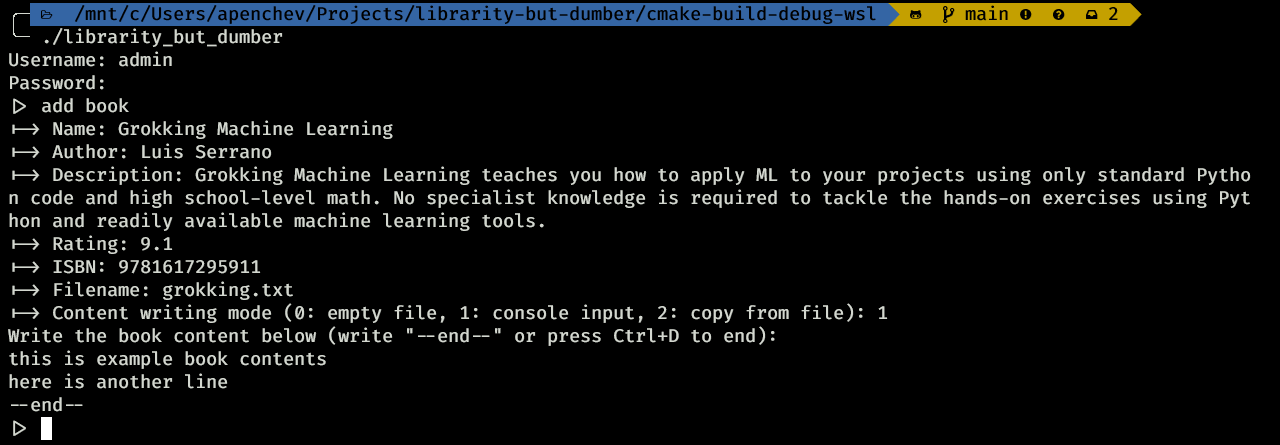
\includegraphics[width=1\textwidth]{4.1.add-book-from-cin.png}
        \centering
        \caption{Добавяне на книга в системата със съдържание от стандартния вход}
        \label{fig:add-book-from-cin}
    \end{figure}
    \begin{figure}[H]
        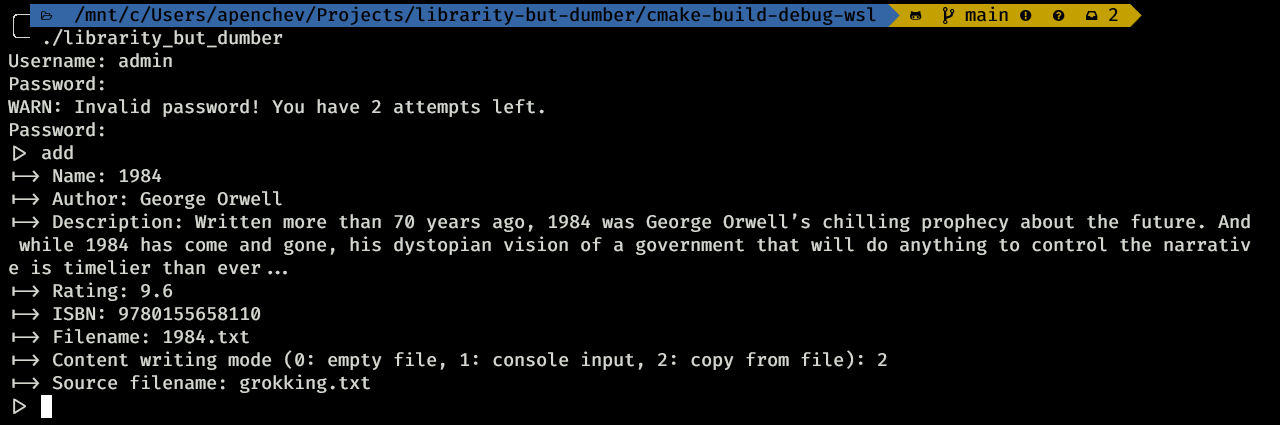
\includegraphics[width=1\textwidth]{4.2.add-book-from-file.png}
        \centering
        \caption{Добавяне на книга в системата със съдържание от текстов файл}
        \label{fig:add-book-from-file}
    \end{figure}
    
    \item Команда за премахване на книга - "remove book" или "remove"
    
    Изисква потедбителят да има администраторски права. Пита потребителя да въведе идентификационния номер (ISBN) на книгата, която да бъде премахната и дали иска да премахне файла със съдържанието на книгата. (Фиг. \ref{fig:remove})
    \begin{figure}[H]
        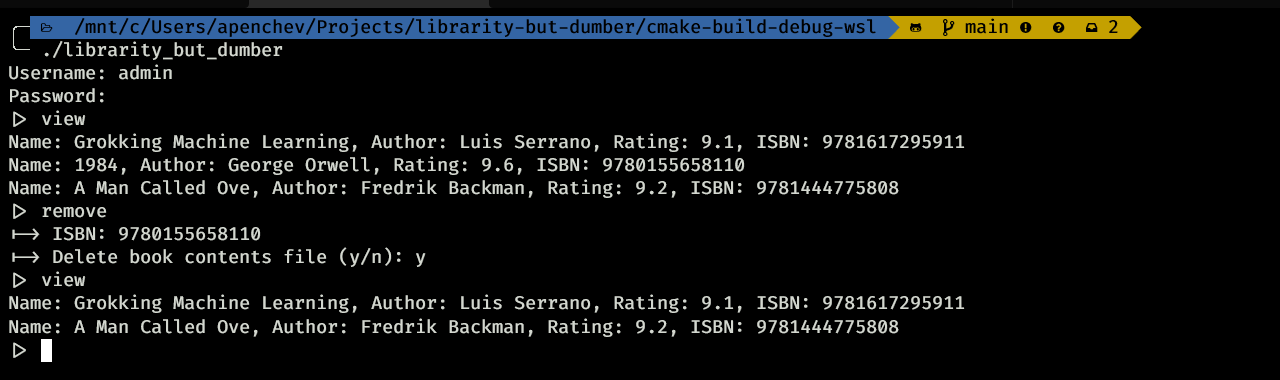
\includegraphics[width=1\textwidth]{5.remove.png}
        \centering
        \caption{Премахване на книга от системата}
        \label{fig:remove}
    \end{figure}
    

    \item Команда за преглед на списък с книгите в системата - "list books", "list" или "view"
    
    Показва всички настоящо добавени книги в системата в неподреден вид. Не изсква допълнителни прараметри. (Фиг. \ref{fig:view})
    \begin{figure}[H]
        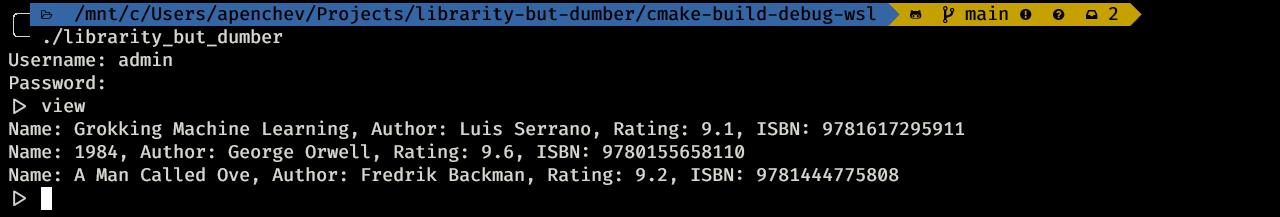
\includegraphics[width=1\textwidth]{6.view.png}
        \centering
        \caption{Преглед на списък с книгите в системата}
        \label{fig:view}
    \end{figure}

    \item Команда за сортиране на книгите в системата - "sort books" или "sort"

    Сортира и показва всички настоящо добавени книги в системата. Изисква от потребителя да избере критерий за сортиране - по име, по автор или по рейтинг. (Фиг. \ref{fig:sort})
    \begin{figure}[H]
        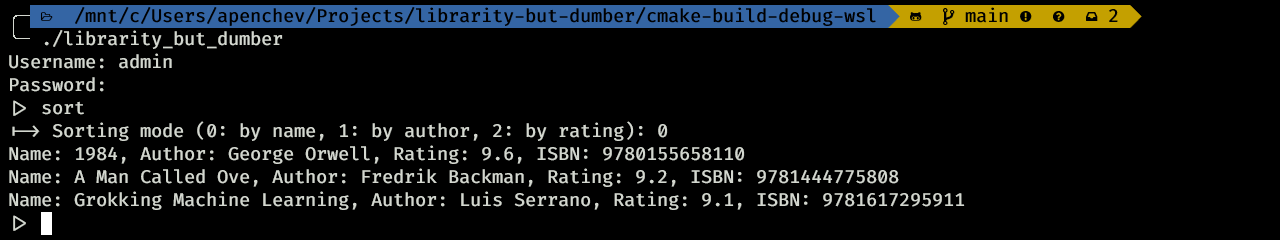
\includegraphics[width=1\textwidth]{7.sort.png}
        \centering
        \caption{Сортиране на книгите в системата}
        \label{fig:sort}
    \end{figure}

    \item Команда за принтиране на книга в системата - "print"
     
    Пита потребителя да въведе идентификационния номер (ISBN) на книгата, която да бъде принтирана. След това изисква да се избере 1 от 3 режима за принтиране - на цялото съдържание, на брой редове, зададени от потребителя, след които се паузира и на отделни изречения. (Фиг. \ref{fig:print})
    \begin{figure}[H]
        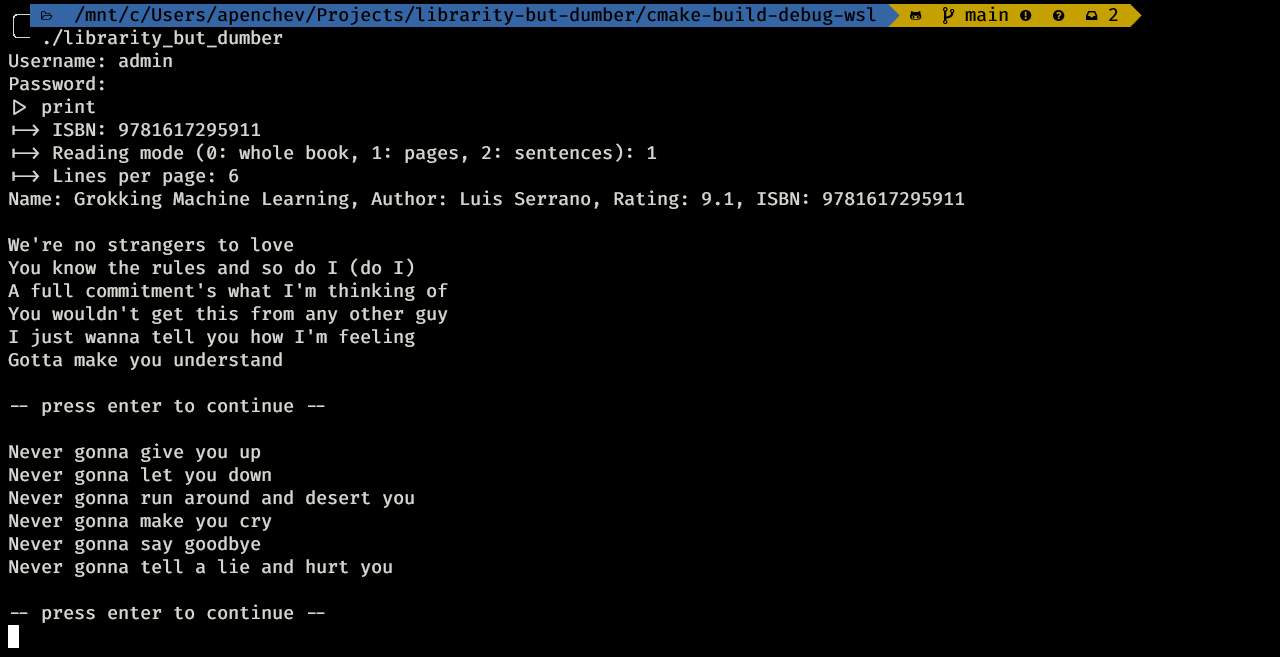
\includegraphics[width=1\textwidth]{8.print.png}
        \centering
        \caption{Принтиране на книга в системата}
        \label{fig:print}
    \end{figure}
\end{enumerate}